\documentclass{article}
\usepackage{graphicx}
\usepackage{listings}
\usepackage[margin=1in]{geometry}
\usepackage{placeins}
\usepackage{float}

\title{Workflow Analytics}
\author{Andrew Smith, Kofi Otseidu, Manav Trivedi}


\begin{document}
\maketitle

\section{Clustering Before and After Settlement}
\subsection{Before Settlement}
Note: We only consider officers who were eventually involved in a settlement of some sort here.

Features are rank, race, gender, number of allegations, age at the time of settlement, and number of awards, respectively. For rank, the encoding is 1-12, generally in order of police hierarchy (1 being officer, 12 being superintendent). For gender, 1 is male, 2 female, and for race, 1 is white, 2 is hispanic, 3 black, 4 Asian, 5 Native American and 6 unknown.


\begin{figure}[h!]
\centering
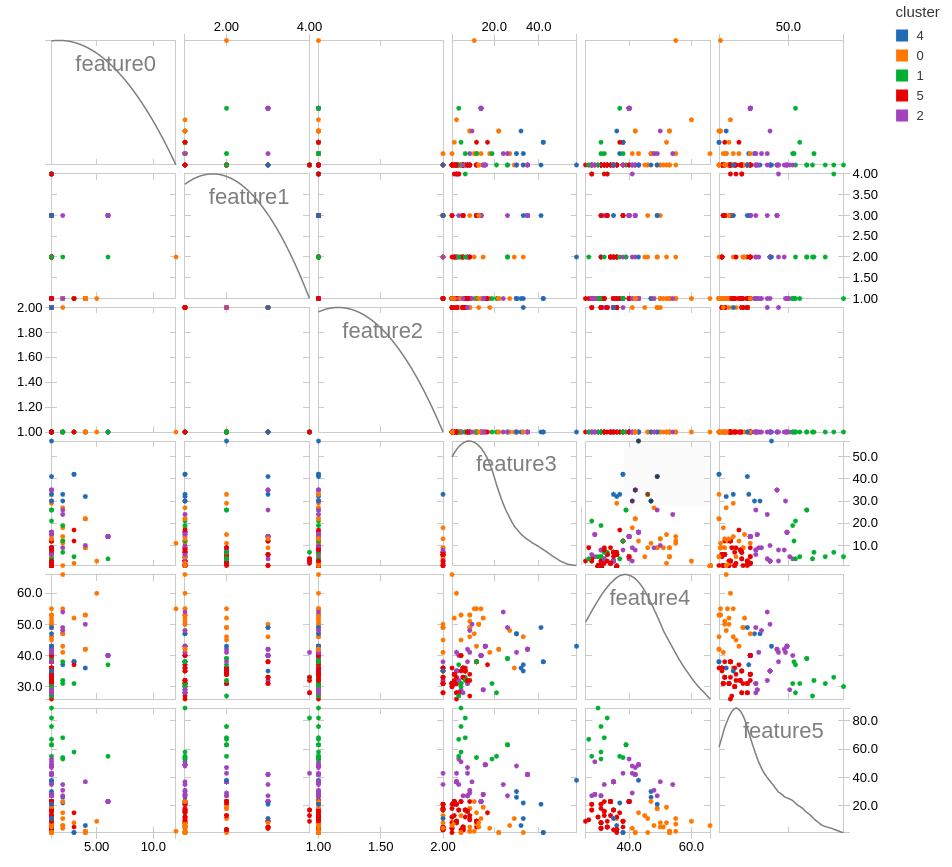
\includegraphics[width=\textwidth]{cluster.png}
\end{figure}
Looking at the clusters, a few patterns emerge:
\begin{enumerate}
\setcounter{enumi}{-1}
\item{A cluster of older officers without many awards}
\item{A cluster of highly decorated young men}
\item{Middle aged men and women officers with quite a few awards}
\item{Middle aged cluster with the most complaints}
\item{Young officers without many awards}
\end{enumerate}
Interestingly, gender, race, and rank don't seem to define the clusters as well as age and awards do, but this may be an effect of the encoding. Rank and age are pretty well correlated, which makes it less useful here.

\FloatBarrier

\subsection{After Settlement}
Keeping the same features and encoding as before, except for the addition of one new feature---a count of the number of settlements the officer was involved in. We also created a column for the total amount of settlement per officer, but the resulting clusters including one single large cluster, so we did not include it.


\begin{figure}[h!]
\centering
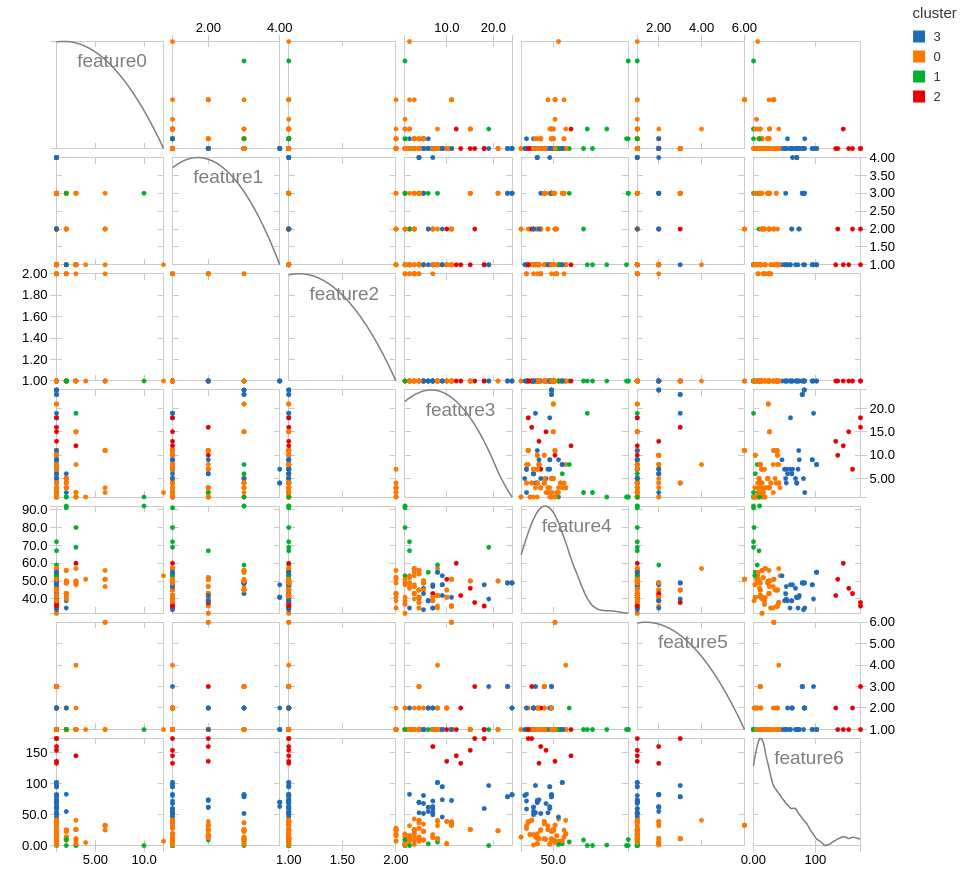
\includegraphics[width=\textwidth]{cluster2.png}
\end{figure}

This time the optimal amount of clusters is four. Just to reiterate, the features are rank, race, gender, number of allegations, age, number of settlements, and awards.
\begin{enumerate}
\setcounter{enumi}{-1}
\item{This cluster is young, without many complaints or awards, also includes more women than any other cluster}
\item{A group of older male officers, without many complaints or awards---Note it looks like this group may include some officers who are no longer in the service, which is why they are so old}
\item{Highly decorated with lots of awards, generally young but also with a decent amount of complaints}
\item{Cluster of young men with some awards and a wide array of complaint numbers}
\end{enumerate}


\section{Are Officers involved in settlements more or less likely to receive complaints in the future?}

Taking the same data from previous question, we can create a box plot for before and after the first settlement an officer is involved in. The plot is below. The median value for before is 10 complaints and for after is 4 complaints. It does, in general, look like being part of a settlement changes an officer's behavior for the better. However, it is also important to note that there are some other factors here. If officers involved in a settlement leave the force, or are sidelined, then they would presumably receive less allegations. Now this isn't a bad thing, in effect police departments are enforcing better behavior, but it isn't quite the same as individual changes in behavior.

\begin{figure}[h!]
\centering
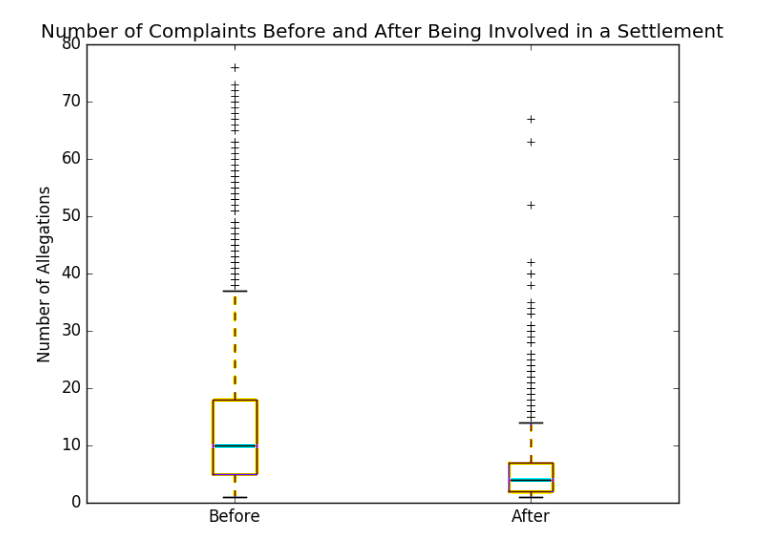
\includegraphics[width=\textwidth]{settb.png}
\end{figure}

\FloatBarrier


\section{Are Neighborhoods where a settlement took place less likely to receive complaints in the future?}


\end{document}